\documentclass[a4paper]{article}
\usepackage[margin=1in]{geometry}
\usepackage{authblk}
\usepackage{graphicx}
\usepackage{hyperref}
\usepackage{biblatex}
\usepackage{algpseudocode}
\usepackage{algorithm}
\usepackage{listings}

\addbibresource{ref.bib}

\title{Cosine Similarity based TopoMap: Update}
\author{Devarsh Patel \\
  \texttt{dp3324@nyu.edu}}
\affil{
  Department of Computer Science \\
  NYU Tandon School of Technnology, NY
}



\begin{document}
  \maketitle

  \begin{center}
    \textbf{Github}: \href{https://github.com/dp3324/advance-topomap}{https://github.com/dp3324/advance-topomap}
  \end{center}

  \begin{abstract}
    The goal of this research is to derive an efficient deviation model for TopoMap algorithm to make it more meaningful. The method used here is derived from Natural Language Processing(NLP) to compare the points similarly how the works are compared using tokenization in NLP.
  \end{abstract}

  \section{Methodology}
  \subsection{Development}
    The implementation of this research is done from scratch in python only by using fundamental datastructures and mathematical libraries. The program is designed in modular fashion built using functional components. The program is designed to run on all type of system architectures. 


  \subsection{Approach}
    The original version of TopoMap\cite{topomap} is based on 3 main features: Euclidian Minimum Spanning Tree, Convex Hull Alignment, Tree Drawing Diagram. This model represented in this research paper is quite efficient for depicting and reducing n-dimensional data into 2-dimension. The model is completely based on the distace relation of the points. There are many other relational models for defining the relation between points like Consine Similarity and Manhattan Distance. After testing this new relationship models on TopoMap\cite{topomap}, I derived at an conclusion that the Cosine Similarity provide better relation between two points than Euclidian distance in given datasets. 
    
    The TopoMap\cite{topomap} algorithm is modified at two points: Minimum Spanning Tree and Convex hull alignment. The original algorithm is the convex hull for the given components and does not consider the alignment of the inner points in the components. It is also heavily dependent on the index of points in the components. To make this more robust, this researh used multi-node branch based hull alogorithm which will include all points inside the hull and at the border to create a tree of an component. The required point in the component is assumed to be the origin and all other points are updated accordingly during rotation along the origin. The sum of all y-coordinates is used as the weight which will be minimize(convex) or maximize(concave) to align the component structure. Later the concave(Cb) component is aligned along the y-axis at the edge point (pb) w.r.t point (pa) from convex (Ca) component such that the d(pa, pb) = e (edge length).

    \newpage
    \subsection{Angle based Minimal Spanning Tree Algorithm}
      \begin{lstlisting}
        Vnew[] = {x}                   
        Enew[] = {}
        while Vnew is not equal to V
            u -> a node from Vnew
            v -> a node that is not in Vnew such that
                 edge u-v has the angle between them
            add v to Vnew
            add edge (u, v) to Enew
        end while
        Return Vnew and Enew
      \end{lstlisting}

      \subsection{Component Alignment PseudoCode \{updated Convex Hull Algorithm\}}
      \begin{lstlisting}
        Cset = [{P1}, {P2},...{Pi}]
        Pa = point of interest in Cset
        weight = null
        for Pi in Cset:
          Pi = Pi - Pa \\ subtract point of interest    
                          from each point
        make weight as max(concave) or min(convex):
          updated_component, weight = rotate(component) \\ rotate by 1 deg
                                                            in each iteration
        for Pi in Cset:
          Pi = Pi + Pa \\ get the original coordinates back
        return updated_component
      \end{lstlisting}
      

  \section{Result}

  TopoMap\cite{topomap} using Cosine Similarity created an amazing results. It was properly able to distinguish the points with respect to their classes and it was also able to bring the outliners more near to their respective class points. The custom convex hull aligment algorithm provided better visual appearance with more gap between clusters tree than original implementation of TopoMap\cite{topomap}.

  The result of using Euclidian Distance and Cosine Similarity with the TopoMap\cite{topomap} algorithm is shown in Figure \ref{iris}. It can be clearly noticed that the are more seperated and distinct which makes their identification easy. Also its worth to notice that the alogorithm provided proper point placement such that no points are completely overlapped each other. While the original implementation of TopoMap provided very close point placement. To verifiy the same, Wine dataset shown in Figure \ref{wine} is used which cleary depicts the above claims.
  
  \cite{topomap}

  \begin{figure}[htb]
    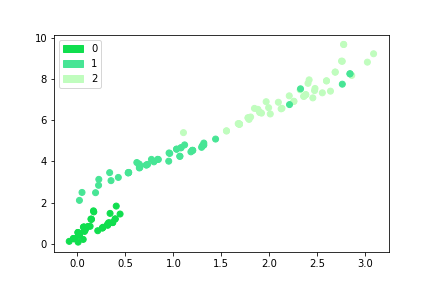
\includegraphics[width=0.5\textwidth]{../output/iris_euclidian_distance_1.png}
    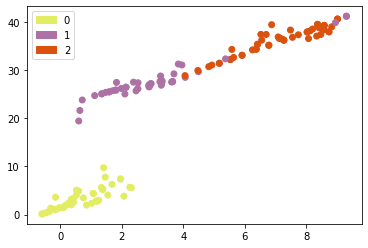
\includegraphics[width=0.5\textwidth]{../output/iris_angle_1.png}
    \caption{Iris dataset output using Euclidian Distance and Cosine Similarity.}
    \label{iris}
  \end{figure}

  \begin{figure}[htb]
    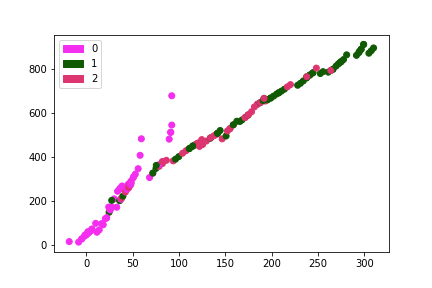
\includegraphics[width=0.5\textwidth]{../output/wine_euclidian_distance_1.png}
    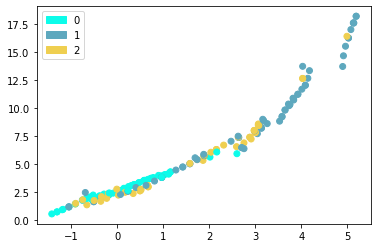
\includegraphics[width=0.5\textwidth]{../output/wine_angle_1.png}
    \caption{Wine dataset output using Euclidian Distance and Cosine Similarity.}
    \label{wine}
  \end{figure}
  
  \newpage
  \printbibliography

\end{document}
